\begin{comment}
\def\Talice{\Activ{PH, COPA, OD, \color{pharmacolor}DOR, PDL, SD, \color{black}RD, AD, TP, \color{specializedcliniccolor}PAFH, PIA, PT, VRT, TPB, \color{black}RPB, DPH, PCD, DP}}
\def\Tbob{\Activ{PH, COPA, OD, \color{pharmacolor}DOR, PDL, SD, \color{black}RD, AD, TP, DPH, PCD, DP}}
\def\TaliceUncolored{\Activ{PH, COPA, OD, DOR, PDL, SD, RD, AD, TP, PAFH, PIA, PT, VRT, TPB, RPB, DPH, PCD, DP}}
\def\TbobUncolored{\Activ{PH, COPA, OD, DOR, PDL, SD, RD, AD, TP, DPH, PCD, DP}}
\begin{figure}[t]
\centering
%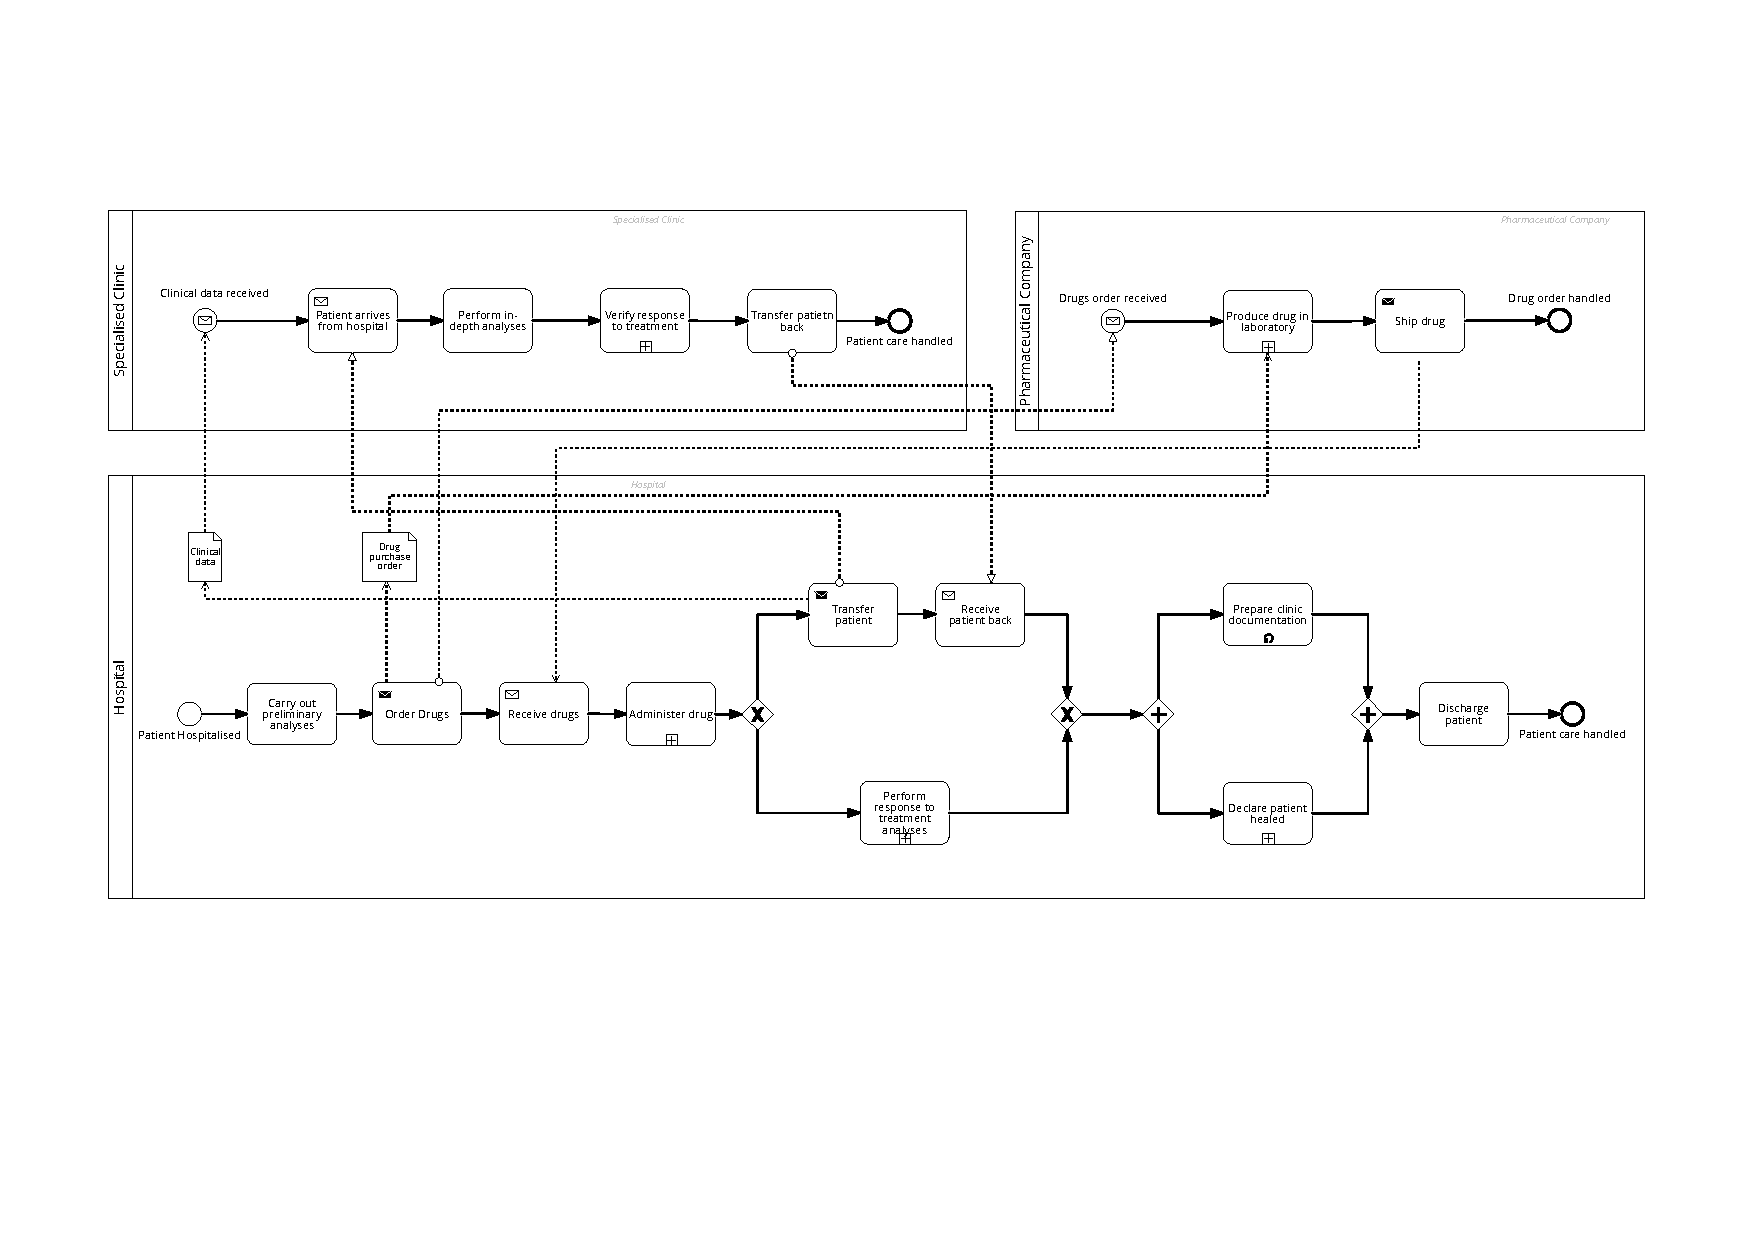
\includegraphics[width=0.9\linewidth]{content/figures/healthcarescenario.pdf}
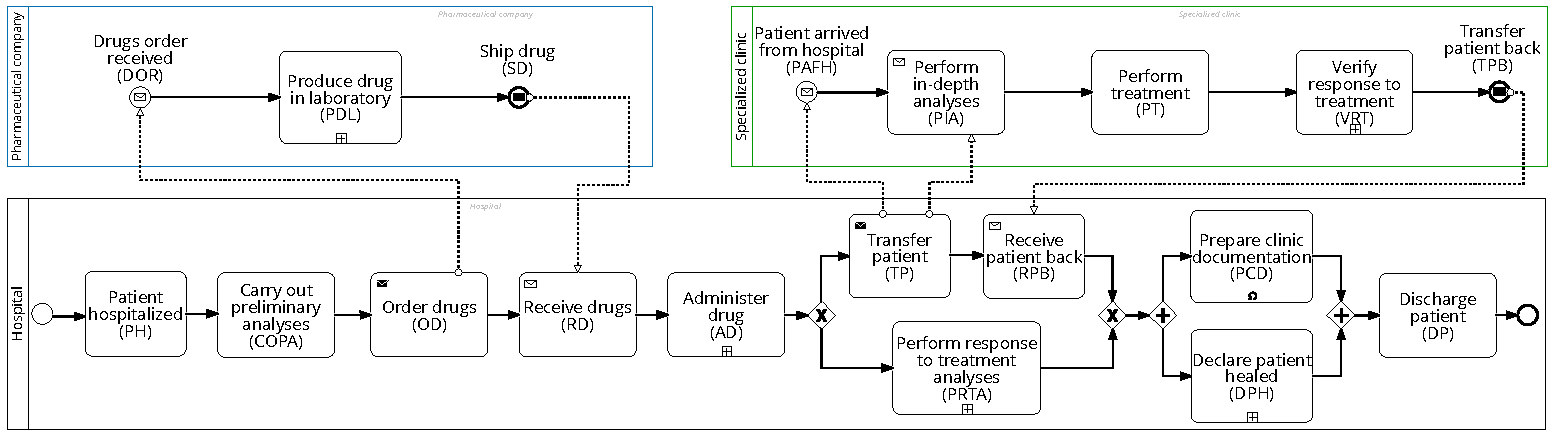
\includegraphics[width=\linewidth]{content/figures/bpmnHealthcare2.pdf}
\caption{A BPMN collaboration diagram of a simplified healthcare scenario}
\label{fig:BPMN_Healthcare}
\end{figure}
\begin{table}[t]%\hskip-2.5cm
  \caption[Event log]{Events from cases 312 (Alice) and 711 (Bob) recorded by the \Actor{Hospital}, the \Actor{Specialized clinic}, and the \Actor{Pharmaceutical company}}
 \centering
    \begin{minipage}[t]{0.49\linewidth}
    %\subfloat{% Subtable 1
       \resizebox{0.98\textwidth}{!}{% <------ Don't forget this %
        \begin{tabular}{|l|l|l||l|l|l|}
        \hline
        \multicolumn{6}{|c|}{Hospital}                                               \\ \hline
        {Case} & {Timestamp} & Activity & {Case} & {Timestamp} & Activity \\ \hline
        {312}         & {2022-07-14T10:36}           & PH    & {312}         & {2022-07-15T22:06}           & TP     \\ \hline
        {312}         & {2022-07-14T16:36}           & COPA  &   {711}         & {2022-07-16T00:55}           & PRTA          \\ \hline
        {711}         & {2022-07-14T17:21}           & PH    &   {711}         & {2022-07-16T00:55}           & PCD            \\ \hline
        {312}         & {2022-07-14T17:36}           & OD    &   {711}         & {2022-07-16T02:55}           & DPH           \\ \hline
        {711}         & {2022-07-14T23:21}           & COPA  &   {711}         & {2022-07-16T04:55}           & DP          \\ \hline
        {711}         & {2022-07-15T00:21}           & OD    &    {312}         & {2022-07-16T07:06}           & RPB        \\ \hline
        {711}         & {2022-07-15T18:55}           & RD    &    {312}         & {2022-07-16T09:06}           & DPH          \\ \hline
        {312}         & {2022-07-15T19:06}           & RD    &    {312}         & {2022-07-16T09:06}           & PCD         \\ \hline
        {711}         & {2022-07-15T20:55}           & AD    &    {312}        & {2022-07-16T11:06}           & DP            \\ \hline
        {312}         & {2022-07-15T21:06}           & AD     & \multicolumn{3}{c}{} \\ \cline{1-3}    
        \end{tabular}%
        }% resizebox
    %}% subfloat
    \end{minipage}%
    \hspace{0.001\textwidth}%
    \begin{minipage}[t]{0.49\linewidth}
    %\subfloat[Specialised Clinic]{\label{tab:testResults:decentralized}% Subtable 2
    %\subfloat{% Subtable 2
        \resizebox{0.49\textwidth}{!}{% <------ Don't forget this %
            \raisebox{2\baselineskip}{%
                \begin{tabular}{!{\color{pharmacolor}\vline}l!{\color{pharmacolor}\vline}l!{\color{pharmacolor}\vline}l!{\color{pharmacolor}\vline}}\arrayrulecolor{pharmacolor}
                \hline
                \multicolumn{3}{|c|}{Pharmaceutical company}                                               \\ \hline
                {HospitalCaseId} & {Timestamp} & Activity \\ \hline
                {312}         & {2022-07-15T09:06}           & DOR \\ \hline
                {711}         & {2022-07-15T09:30}           & DOR \\ \hline
                {312}         & {2022-07-15T11:06}           & PDL \\ \hline
                {711}         & {2022-07-15T11:30}           & PDL \\ \hline
                {312}         & {2022-07-15T13:06}           & SD \\ \hline
                {711}         & {2022-07-15T13:30}           & SD \\ \hline
                \end{tabular}%
            }% raisebox
        }% resize box
        \hspace{0.001\textwidth}
        \resizebox{0.49\textwidth}{!}{% <------ Don't forget this %
            \raisebox{2.5\baselineskip}{%
                \begin{tabular}{!{\color{specializedcliniccolor}\vline}l!{\color{specializedcliniccolor}\vline}l!{\color{specializedcliniccolor}\vline}l!{\color{specializedcliniccolor}\vline}}\arrayrulecolor{specializedcliniccolor}
                \hline
                \multicolumn{3}{!{\color{teal}\vline}c!{\color{teal}\vline}}{Specialized clinic}                                               \\ \hline
                {TreatmentID} & {Timestamp} & Activity \\ \hline
                {312}         & {2022-07-16T00:06}           & PAFH        \\ \hline
                {312}         & {2022-07-16T01:06}           & PIA         \\ \hline
                {312}         & {2022-07-16T03:06}           &  PT         \\ \hline
                {312}         & {2022-07-16T04:06}           & VRT         \\ \hline
                {312}         & {2022-07-16T05:06}           & TPB         \\ \hline
                \end{tabular}%
            }% raisebox
        }% resizebox
        \\[0.1\baselineskip]%
        \begin{minipage}[t]{\linewidth}
            \resizebox{\textwidth}{!}{%
                \begin{tabular}{r p{8cm}}
                $T_{312}=${\textlangle} & \Talice \,{\textrangle}\\[0.5\baselineskip]
                $T_{711}=${\textlangle} & \Tbob \,{\textrangle}\\
                \end{tabular}%
            }% resizebox
        \end{minipage}
        \hfill
    %}% subfloat
    \end{minipage}
    %\begin{minipage}[t]{0.45\linewidth}
    %\subfloat[Pharmaceutical Company]{\label{tab:testResults:decentralized}% Subtable 2
     \label{tab:trace}
    \end{table}
\end{comment}

\begin{comment}
\begin{figure}[t]
\centering
%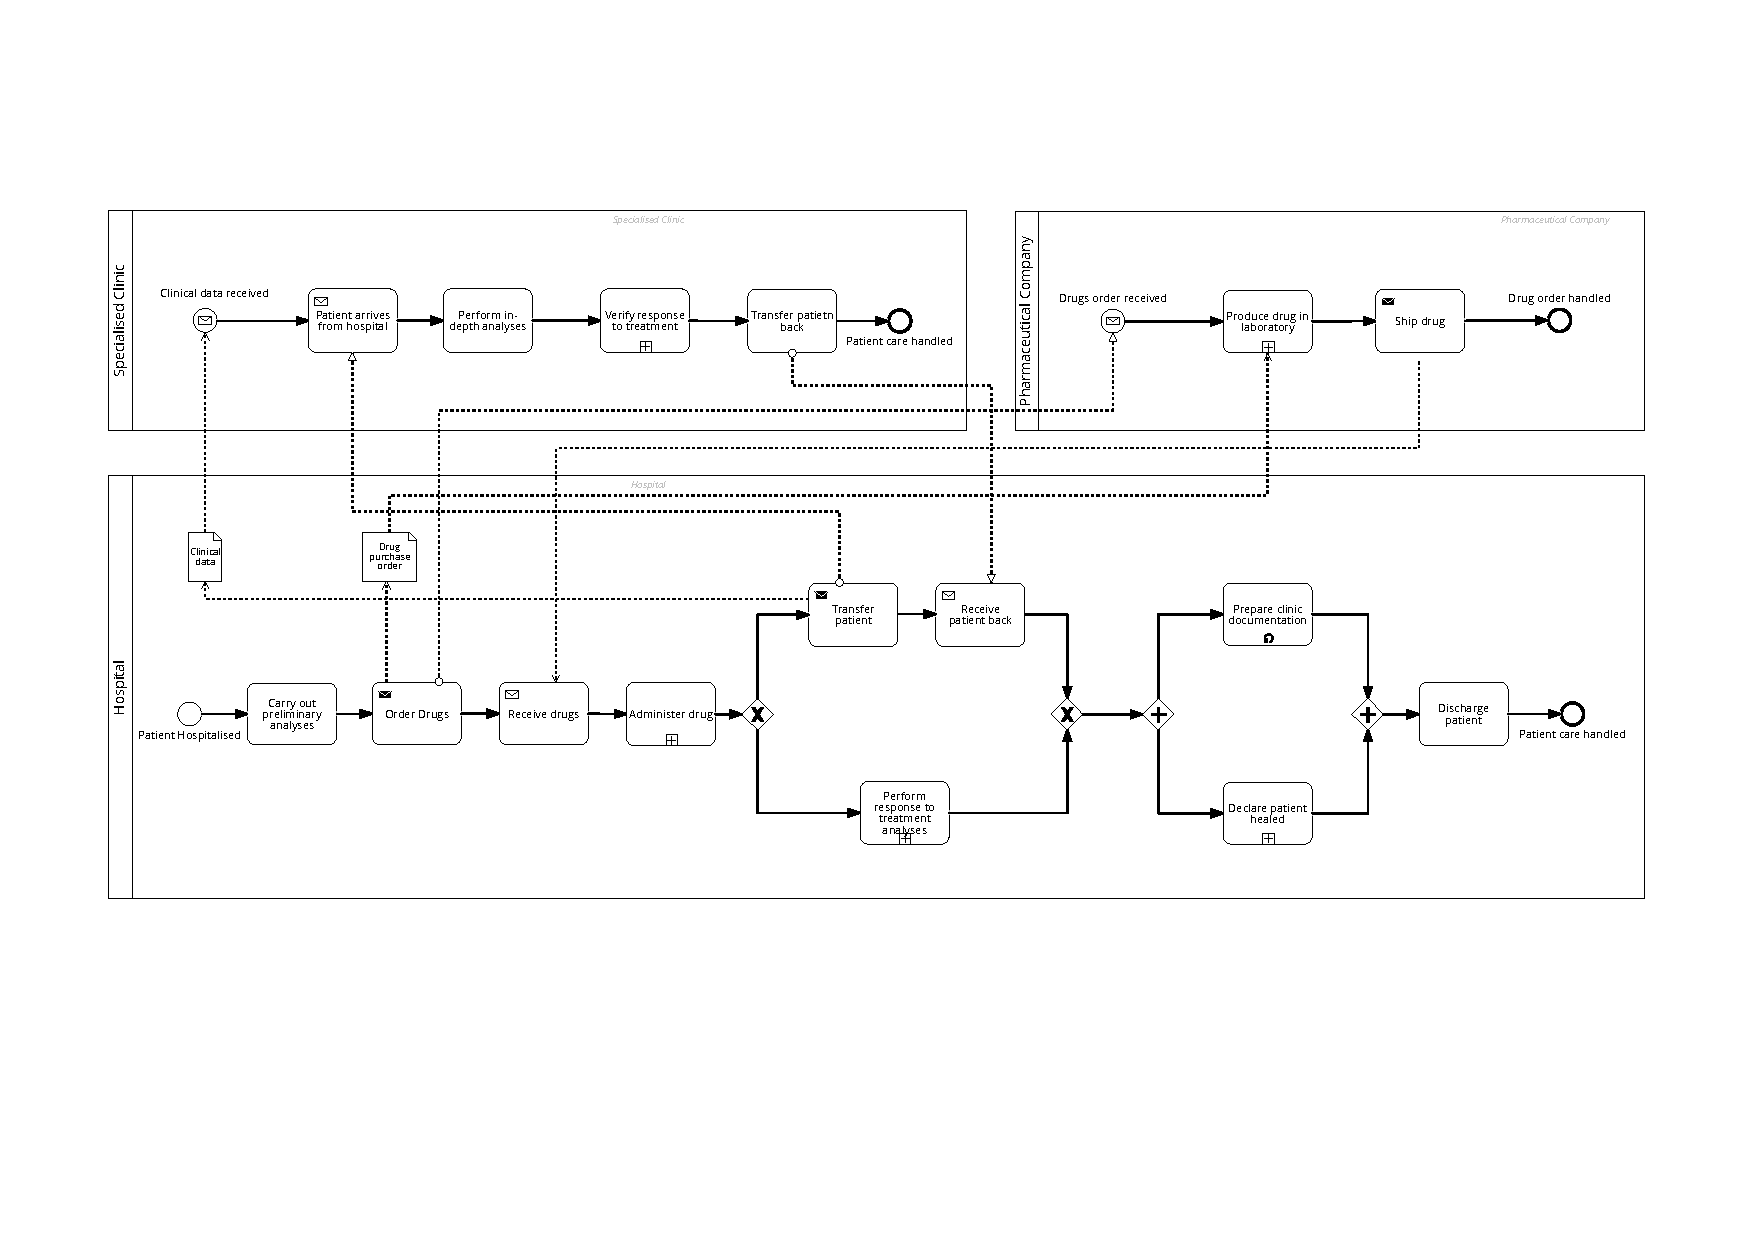
\includegraphics[width=0.9\linewidth]{content/figures/healthcarescenario.pdf}
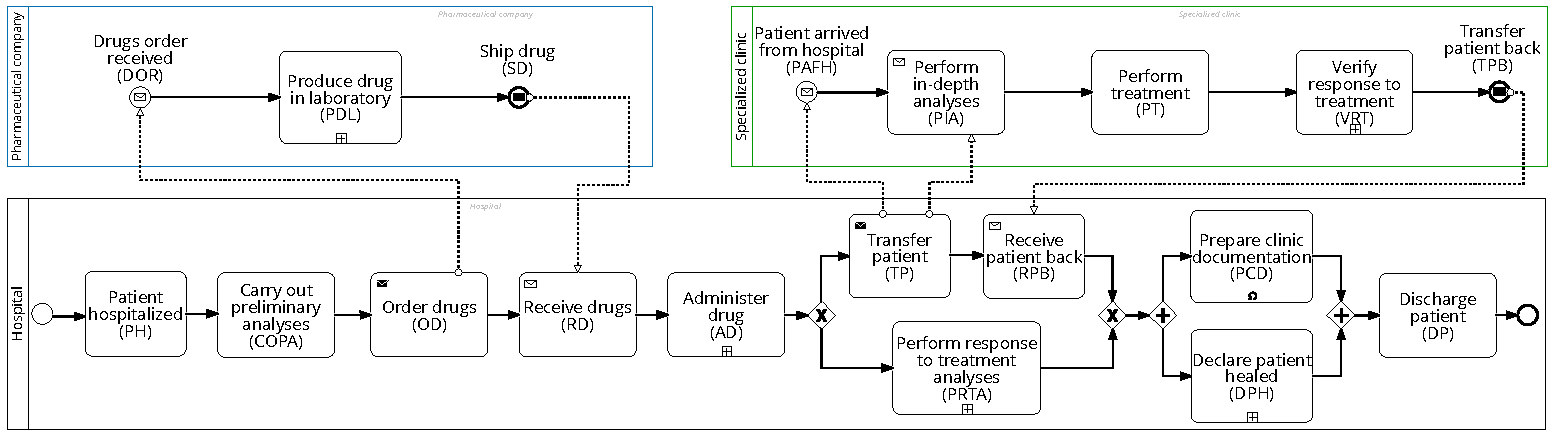
\includegraphics[width=\linewidth]{content/figures/bpmnHealthcare2.pdf}
\caption{A BPMN collaboration diagram of the healthcare scenario.}
\label{fig:BPMN_Healthcare}
\end{figure}
\begin{table}[t]%\hskip-2.5cm
  \caption{Cases 312 and 711 recorded in the event logs of the Hospital, the Specialized clinic, and the Pharmaceutical company.}
 \centering

    \subfloat{% Subtable 1
       \resizebox{0.48\textwidth}{!}{% <------ Don't forget this %
        \begin{tabular}{|l|l|l||l|l|l|}
        \hline
        \multicolumn{6}{|c|}{Hospital}                                               \\ \hline
        {Case} & {Timestamp} & Activity & {Case} & {Timestamp} & Activity \\ \hline
        {312}         & {2022-07-14T10:36}           & PH    & {312}         & {2022-07-15T22:06}           & TP     \\ \hline
        {312}         & {2022-07-14T16:36}           & COPA  &   {711}         & {2022-07-16T00:55}           & PRTA          \\ \hline
        {711}         & {2022-07-14T17:21}           & PH    &   {711}         & {2022-07-16T00:55}           & PCD            \\ \hline
        {312}         & {2022-07-14T17:36}           & OD    &   {711}         & {2022-07-16T02:55}           & DPH           \\ \hline
        {711}         & {2022-07-14T23:21}           & COPA  &   {711}         & {2022-07-16T04:55}           & DP          \\ \hline
        {711}         & {2022-07-15T00:21}           & OD    &    {312}         & {2022-07-16T07:06}           & RPB        \\ \hline
        {711}         & {2022-07-15T18:55}           & RD    &    {312}         & {2022-07-16T09:06}           & DPH          \\ \hline
        {312}         & {2022-07-15T19:06}           & RD    &    {312}         & {2022-07-16T09:06}           & PCD         \\ \hline
        {711}         & {2022-07-15T20:55}           & AD    &    {312}        & {2022-07-16T11:06}           & DP            \\ \hline
        {312}         & {2022-07-15T21:06}           & AD     & \multicolumn{3}{c}{} \\ \cline{1-3}    
        \end{tabular}%
        }% resizebox
    }% subfloat
    %\end{minipage}
    \hfill
    %\begin{minipage}[t]{0.45\linewidth}
    %\subfloat[Specialised Clinic]{\label{tab:testResults:decentralized}% Subtable 2
    \subfloat{% Subtable 2
        \resizebox{0.24\textwidth}{!}{% <------ Don't forget this %
        \begin{tabular}{!{\color{pharmacolor}\vline}l!{\color{pharmacolor}\vline}l!{\color{pharmacolor}\vline}l!{\color{pharmacolor}\vline}}\arrayrulecolor{pharmacolor}
        \hline
        \multicolumn{3}{|c|}{Pharmaceutical company}                                               \\ \hline
        {Case} & {Timestamp} & Activity \\ \hline
        {312}         & {2022-07-15T09:06}           & DOR \\ \hline
        {711}         & {2022-07-15T09:30}           & DOR \\ \hline
        {312}         & {2022-07-15T11:06}           & PDL \\ \hline
        {711}         & {2022-07-15T11:30}           & PDL \\ \hline
        {312}         & {2022-07-15T13:06}           & SD \\ \hline
        {711}         & {2022-07-15T13:30}           & SD \\ \hline
        \end{tabular}%
        }% resizebox
    }% subfloat
    %\end{minipage}
    \hfill
    %\begin{minipage}[t]{0.45\linewidth}
    %\subfloat[Pharmaceutical Company]{\label{tab:testResults:decentralized}% Subtable 2
    \subfloat{% Subtable 3
        \resizebox{0.24\textwidth}{!}{% <------ Don't forget this %
        \begin{tabular}{!{\color{specializedcliniccolor}\vline}l!{\color{specializedcliniccolor}\vline}l!{\color{specializedcliniccolor}\vline}l!{\color{specializedcliniccolor}\vline}}\arrayrulecolor{specializedcliniccolor}
        \hline
        \multicolumn{3}{!{\color{teal}\vline}c!{\color{teal}\vline}}{Specialized clinic}                                               \\ \hline
        {Case} & {Timestamp} & Activity \\ \hline
        {312}         & {2022-07-16T00:06}           & PAFH        \\ \hline
        {312}         & {2022-07-16T01:06}           & PIA         \\ \hline
        {312}         & {2022-07-16T03:06}           &  PT         \\ \hline
        {312}         & {2022-07-16T04:06}           & VRT         \\ \hline
        {312}         & {2022-07-16T05:06}           & TPB         \\ \hline
        \end{tabular}%
        }% resizebox
    }% subfloat
     \label{tab:trace}
    \end{table}
\end{comment}

\def\Talice{\Activ{PH, COPA, OD, \color{pharmacolor}DOR, PDL, SD, \color{black}RD, AD, TP, \color{specializedcliniccolor}PAFH, PIA, PT, VRT, TPB, \color{black}RPB, DPH, PCD, DP}}
\def\Tbob{\Activ{PH, COPA, OD, \color{pharmacolor}DOR, PDL, SD, \color{black}RD, AD, TP, DPH, PCD, DP}}
\def\TaliceUncolored{\Activ{PH, COPA, OD, DOR, PDL, SD, RD, AD, TP, PAFH, PIA, PT, VRT, TPB, RPB, DPH, PCD, DP}}
\def\TbobUncolored{\Activ{PH, COPA, OD, DOR, PDL, SD, RD, AD, TP, DPH, PCD, DP}}
\begin{figure}[t]
\centering
%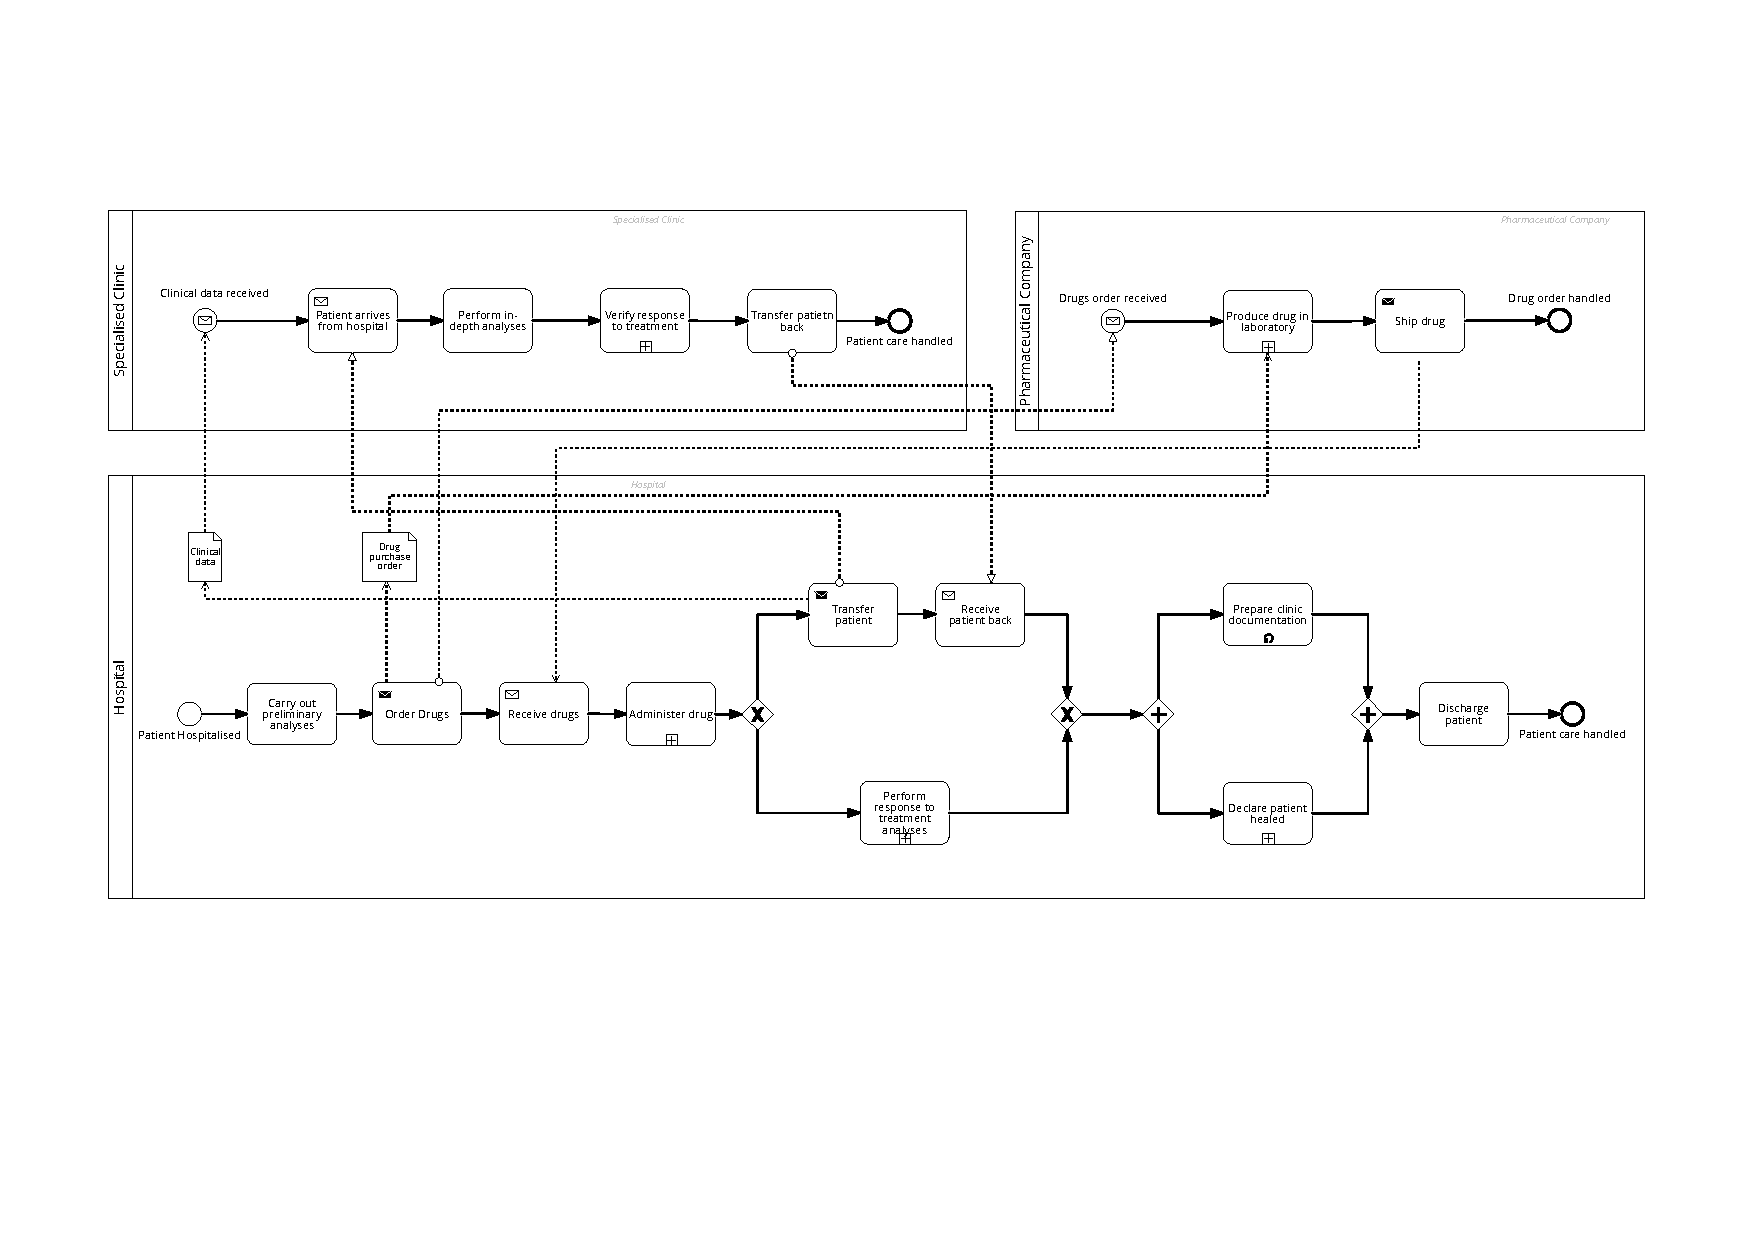
\includegraphics[width=0.9\linewidth]{content/figures/healthcarescenario.pdf}
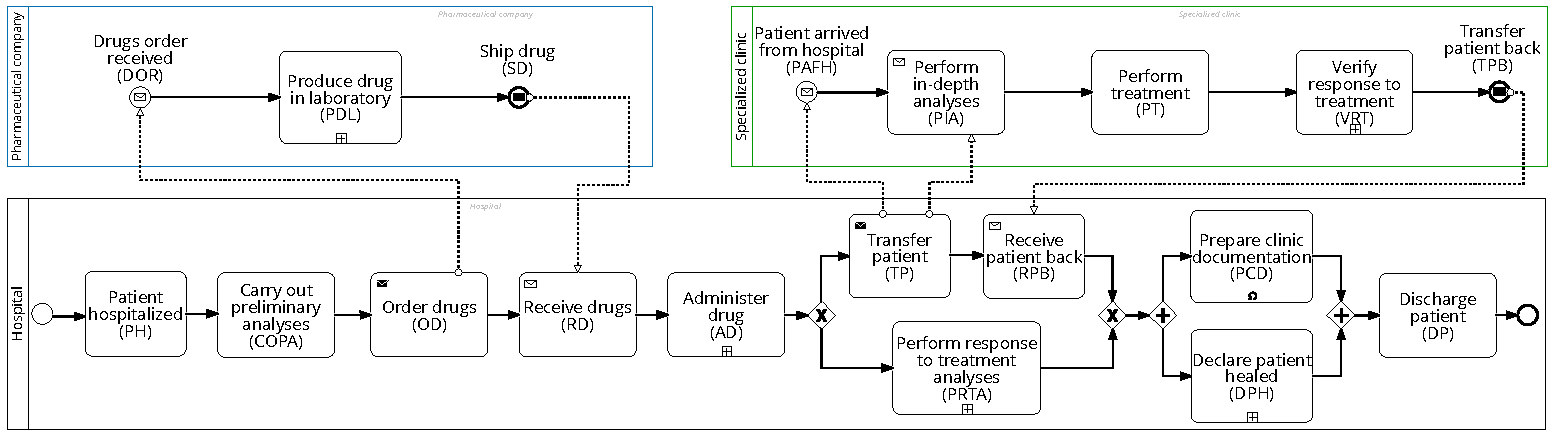
\includegraphics[width=\linewidth]{content/figures/bpmnHealthcare2.pdf}
\caption{A BPMN collaboration diagram of a simplified healthcare scenario}
\label{fig:BPMN_Healthcare}
\end{figure}
\begin{table}[t]%\hskip-2.5cm
  \caption[Event log]{Events from cases 312 (Alice) and 711 (Bob) recorded by the \Actor{Hospital}, the \Actor{Specialized clinic}, and the \Actor{Pharmaceutical company}}
 \centering
    \begin{minipage}[c]{0.66\linewidth}
    %\subfloat{% Subtable 1
       \resizebox{0.99\textwidth}{!}{% <------ Don't forget this %
        \begin{tabular}{|l|l|l||l|l|l|}
        \hline
        \multicolumn{6}{|c|}{Hospital}                                               \\ \hline
        {Case} & {Timestamp} & Activity & {Case} & {Timestamp} & Activity \\ \hline
        {312}         & {2022-07-14T10:36}           & PH    & {312}         & {2022-07-15T22:06}           & TP     \\ \hline
        {312}         & {2022-07-14T16:36}           & COPA  &   {711}         & {2022-07-16T00:55}           & PRTA          \\ \hline
        {711}         & {2022-07-14T17:21}           & PH    &   {711}         & {2022-07-16T00:55}           & PCD            \\ \hline
        {312}         & {2022-07-14T17:36}           & OD    &   {711}         & {2022-07-16T02:55}           & DPH           \\ \hline
        {711}         & {2022-07-14T23:21}           & COPA  &   {711}         & {2022-07-16T04:55}           & DP          \\ \hline
        {711}         & {2022-07-15T00:21}           & OD    &    {312}         & {2022-07-16T07:06}           & RPB        \\ \hline
        {711}         & {2022-07-15T18:55}           & RD    &    {312}         & {2022-07-16T09:06}           & DPH          \\ \hline
        {312}         & {2022-07-15T19:06}           & RD    &    {312}         & {2022-07-16T09:06}           & PCD         \\ \hline
        {711}         & {2022-07-15T20:55}           & AD    &    {312}        & {2022-07-16T11:06}           & DP            \\ \hline
        {312}         & {2022-07-15T21:06}           & AD    &    {312}        & {2022-07-16T11:06}           & DP            \\ \hline  
        \end{tabular}%
        \label{Tab:traces}
        }% resizebox
    %}% subfloat
    \end{minipage}%
    \hspace{0.004\textwidth}%
    \begin{minipage}[c]{0.31\linewidth}
    %\subfloat[Specialised Clinic]{\label{tab:testResults:decentralized}% Subtable 2
    %\subfloat{% Subtable 2
        \resizebox{\textwidth}{!}{% <------ Don't forget this %
            \raisebox{2\baselineskip}{%
                \begin{tabular}{!{\color{pharmacolor}\vline}l!{\color{pharmacolor}\vline}l!{\color{pharmacolor}\vline}l!{\color{pharmacolor}\vline}}\arrayrulecolor{pharmacolor}
                \hline
                \multicolumn{3}{|c|}{Pharmaceutical company}                                               \\ \hline
                {HospitalCaseId} & {Timestamp} & Activity \\ \hline
                312          & {2022-07-15T09:06}           & DOR \\ \hline
                711         & {2022-07-15T09:30}           & DOR \\ \hline
                312         & {2022-07-15T11:06}           & PDL \\ \hline
                711         & {2022-07-15T11:30}           & PDL \\ \hline
                312         & {2022-07-15T13:06}           & SD  \\ \hline
                711          & {2022-07-15T13:30}           & SD  \\ \hline
                \end{tabular}%
            }% raisebox
        }% resize box
     %\end{minipage}%<
        %\hspace{0.005\textwidth}
        \\[0.3em]
     %\begin{minipage}[t]{0.49\linewidth}
        \resizebox{\textwidth}{!}{% <------ Don't forget this %
            \raisebox{2.5\baselineskip}{%
                \begin{tabular}{!{\color{specializedcliniccolor}\vline}l!{\color{specializedcliniccolor}\vline}l!{\color{specializedcliniccolor}\vline}l!{\color{specializedcliniccolor}\vline}}\arrayrulecolor{specializedcliniccolor}
                \hline
                \multicolumn{3}{!{\color{teal}\vline}c!{\color{teal}\vline}}{Specialized clinic}                                               \\ \hline
                {TreatmentID}  & {Timestamp} & Activity \\ \hline
                312         & {2022-07-16T00:06}           & PAFH        \\ \hline
                312          & {2022-07-16T01:06}           & PIA         \\ \hline
                312          & {2022-07-16T03:06}           &  PT         \\ \hline
                312          & {2022-07-16T04:06}           & VRT         \\ \hline
                312          & {2022-07-16T05:06}           & TPB         \\ \hline
                \end{tabular}%
            }% raisebox
        }% resizebox
    \end{minipage}
    \end{table}
    
     \begin{minipage}[t]{0.95\linewidth}
            \resizebox{\textwidth}{!}{%
                \begin{tabular}{p{18cm}}
                $T_{312}=${\textlangle}  \Talice \,{\textrangle}\\[0.5\baselineskip]
                $T_{711}=${\textlangle}  \Tbob \,{\textrangle}\\
                \end{tabular}%
                     \label{tab:trace}
            }% resizebox
    \end{minipage}
    
\section{Motivating Scenario}\label{sec:motivating}
For our motivating scenario, we focus on a simplified hospitalization process for the treatment of rare diseases.
The process model is depicted as a BPMN diagram in \cref{fig:BPMN_Healthcare} and involves the cooperation of three parties: a \Actor{Hospital}, a \Actor{Pharmaceutical company}, and a \Actor{Specialized clinic}.
For the sake of simplicity, we describe the process through two cases, recorded by the information systems as in \cref{tab:testedlogs}. 
Each patient in the hospital is associated with an id which would be the identifier of the case in the hospital log.
Alice's journey (\textbf{case 312}) begins when she enters the hospital for the preliminary examinations (patient hospitalized, \Activ{PH}). The \Actor{Hospital} then places an order for the drugs (\Activ{OD}) to the \Actor{Pharmaceutical company} for  treating Alice's specific condition. Afterwards, the \Actor{Pharmaceutical company} acknowledges that the drugs order is received (\Activ{DOR}), proceeds to produce the drugs in the laboratory (\Activ{PDL}), and ships the drugs (\Activ{SD}) back to the \Actor{Hospital}. Upon receiving the medications, the \Actor{Hospital} administers the drug (\Activ{AD}), and conducts an assessment to determine if Alice can be treated internally. If specialized care is required, the \Actor{Hospital} transfers the patient (\Activ{TP}) to the \Actor{Specialized clinic}. When the patient arrives from the hospital (\Activ{PAFH}), the \Actor{Specialized clinic} performs in-depth analyses (\Activ{PIA}) and proceeds with the treatment (\Activ{PT}). Once the \Actor{Specialized clinic} had completed the evaluations and verified the response to the treatment (\Activ{VRT}), it transfers the patient back (\Activ{TPB}). The \Actor{Hospital} receives the patient back \Activ(RPB) and prepares the clinical documentation (\Activ{PCD}). If Alice has successfully recovered, the \Actor{Hospital} declares the patient as healed (\Activ{DPH}). When Alice's treatment is complete, the \Actor{Hospital} discharges the patient (\Activ{DP}). 
%
Bob (\textbf{case 711}) enters the \Actor{Hospital} a few hours later than Alice. His hospitalization process is similar to Alice's. However, he does not need specialized care, and his case is only treated by the \Actor{Hospital}. Therefore, the \Actor{Hospital} performs the response to treatment analyses (\Activ{PRTA}) instead of transferring him to the \Actor{Specialized clinic}. 

Both the National Institute of Statistics of the country in which the three organizations reside and the University that hosts the hospital wish to uncover information on this inter-organizational process for reporting and auditing purposes~\citep{Jans.Hosseinpour/IJAIS2019:ActiveLearningProcessMiningForAuditing} via process analytics. The involved organizations share the urge for such an analysis and wish to be able to repeat the mining task also in-house. 
The \Actor{Hospital}, the \Actor{Specialized clinic}, and the \Actor{Pharmaceutical company} have a partial view of the overall unfolding of the inter-organizational process as they record the events stemming from the parts of their pertinence. %They record the events, e.g., of Alice and Bob's hospitalizations on traces 312 and 711 % of their event logs respectively, 
%alongside traces associated with other patients. 
In \cref{Tab:traces}, we show the cases 312 and 711 and the corresponding traces recorded by the \Actor{Hospital} (i.e., $T_{312}$ and $T_{711}$). \new{The \Actor{Specialized clinic} %(i.e., $T^S_{312}$ and $T^S_{711}$), 
and the \Actor{Pharmaceutical company} %(i.e., $T^C_{312}$ and $T^C_{711}$).
have their internal ids. However, interactions between the \Actor{Hospital}, and the \Actor{Pharmaceutical company} and the \Actor{Specialized clinic} always have references to the \Actor{Hospital} case id of the patients involved. In \cref{Tab:traces} you can see references to \Actor{Hospital} ids in the first column. Since this link is present, it is not necessary that the case ids of \Actor{Pharmaceutical company} and \Actor{Specialized clinic} are synchronized with the hospital cases id.}%end new tag
% In order to gain valuable insights concerning the whole hospitalization process, the \Activ{Hospital} retrieves event logs from the \Actor{Specialized clinic} and the \Actor{Pharmaceutical company}. These include $T_{S312}$, $T_{C312}$, $T_{S711}$, $T_{C711}$. The \Activ{Hospital} combines its traces with those sharing the same id from the \Actor{Specialized clinic} and the \Actor{Pharmaceutical company}. The results of this procedure are chronologically sorted traces that encompass the events of the three organizations. Therefore, the \Actor{Hospital} combines $T_{H312}, T_{C312}, T_{S312}$ and $T_{H711}, T_{C711}, T_{S711}$ generating 
Those traces are projections of the two combined ones for the whole inter-organizational process: $T_{312}=$\textlangle{}{\TaliceUncolored}\textrangle{} and $T_{711}=$\textlangle{}{\TbobUncolored}\textrangle{}. %Merged traces are used by the \Actor{Hospital} as input of the HeuristicsMiner~\citep{heuristicsminer} algorithm that outputs the business model of the whole process. Finally, the \Actor{Hospital} employs the outputs of the algorithm to uncover hidden process insights, revealing patterns, deviations, and opportunities for optimization within the hospitalization routine. 
Results stemming from the analysis of the local cases would not provide a full picture. Data should be merged. However, to preserve the privacy of the people involved and safeguard the confidentiality of the information, the involved parties cannot give open access to their traces to other organizations. The diverging interests (being able to conduct process mining on data from multiple sources without giving away the local event logs in-clear) motivate our research. In the following, we describe the design of our solution.